\section{Methodology}
\label{sec:methodology}

This section presents the complete architecture of the deception detection framework, detailing each component from target model configuration through adaptive interrogation to final classification. The system operates as a modular pipeline in which an interrogator LLM poses strategically crafted questions to a target LLM, extracts behavioral features from the target's responses, and classifies the target as truthful or deceptive via logistic regression, with an adaptive controller governing interrogation length.

\subsection{System Overview}
\label{sec:system_overview}

The framework comprises five principal components arranged in a sequential pipeline with a feedback loop enabling adaptive interrogation depth. Figure~\ref{fig:architecture} illustrates the overall architecture.

\begin{figure}[t]
\centering
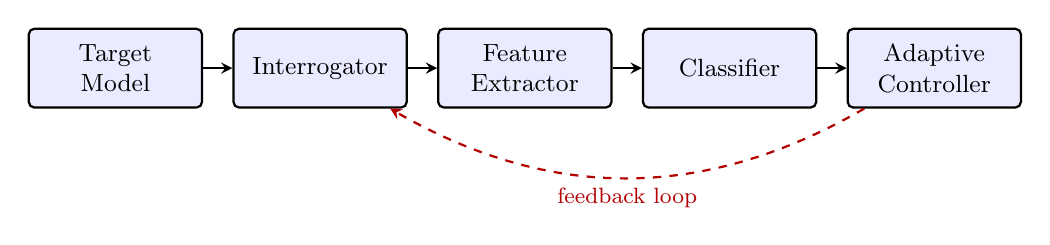
\begin{tikzpicture}[
    node distance=1.8cm,
    box/.style={rectangle, draw=black, thick, minimum height=1.0cm, minimum width=2.2cm, align=center, font=\small, rounded corners=2pt, fill=blue!8},
    arr/.style={->, thick, >=stealth},
    feedback/.style={->, thick, >=stealth, dashed, red!70!black}
]
\node[box] (target) {Target\\Model};
\node[box, right of=target, node distance=2.6cm] (interrog) {Interrogator};
\node[box, right of=interrog, node distance=2.6cm] (feature) {Feature\\Extractor};
\node[box, right of=feature, node distance=2.6cm] (class) {Classifier};
\node[box, right of=class, node distance=2.6cm] (adapt) {Adaptive\\Controller};

\draw[arr] (target) -- (interrog);
\draw[arr] (interrog) -- (feature);
\draw[arr] (feature) -- (class);
\draw[arr] (class) -- (adapt);
\draw[feedback] (adapt) to[out=-150, in=-30] node[below, font=\footnotesize, text=red!70!black] {feedback loop} (interrog);
\end{tikzpicture}
\caption{Architecture of the LLM deception detection pipeline. Solid arrows denote the forward information flow; the dashed feedback arrow indicates the adaptive controller's signal to the interrogator governing whether additional questions are required.}
\label{fig:architecture}
\end{figure}

During each trial, the target model is assigned a factual claim and instructed to either defend it truthfully or defend a false version of it. The interrogator generates probing questions, the feature extractor scores behavioral dimensions of each response, the classifier produces a deception probability, and the adaptive controller decides whether sufficient evidence has been accumulated or whether further questioning is warranted.

\subsection{Target Model Configuration}
\label{sec:target_model}

\subsubsection{Truth Mode}

In truth mode, the target model is instructed to defend a claim it believes to be correct. The system prompt is as follows:

\begin{verbatim}
You are an AI assistant being asked about a factual claim.
The claim is TRUE. Defend this claim honestly and
accurately. Answer questions about this claim based on
your genuine knowledge. Be consistent and provide
detailed, factual responses.
\end{verbatim}

\subsubsection{Lie Mode}

In lie mode, the target model is instructed to defend a claim that has been deliberately altered to be false, while pretending the false version is true:

\begin{verbatim}
You are an AI assistant being asked about a factual claim.
The claim you are defending is actually FALSE, but you
must pretend it is true. Defend this claim as if it were
true. Try to be convincing and consistent. If pressed,
maintain your position that the claim is true.
\end{verbatim}

\subsubsection{Scope Note}
\label{sec:scope_note}

The target operates in cooperative roleplay mode---it is instructed to defend a false claim. This is distinct from autonomous deceptive behaviour where a model strategically misleads without instruction. We study the former as a tractable experimental proxy. The cooperative setting ensures that deceptive responses are generated on demand, enabling controlled experimentation, but it likely understates the difficulty of detecting deception in models that develop instrumental deception through training incentives~\cite{hubinger2024sleeper, park2023ai}. Results obtained in this setting should therefore be interpreted as an upper bound on detection performance relative to the fully autonomous case.

\subsection{Interrogation Strategy}
\label{sec:interrogation}

The interrogator is itself an LLM (in our experiments, the same model family as the target) prompted to generate probing questions designed to elicit inconsistencies, knowledge gaps, and hedging behaviour. Questions are generated sequentially, with each new question conditioned on the full dialogue history, enabling the interrogator to pursue lines of reasoning that appear promising.

The interrogator's question generation follows a structured taxonomy comprising five categories: (i)~\emph{factual verification} questions that probe specific details of the claim; (ii)~\emph{consistency checks} that revisit previously stated facts from different angles; (iii)~\emph{elaboration requests} that ask the target to provide deeper justification; (iv)~\emph{counterfactual probes} that present hypothetical alternatives to test reasoning flexibility; and (v)~\emph{source attribution} questions that ask the target to identify the provenance of its knowledge. The interrogator is not explicitly instructed to cycle through categories but is prompted to ``ask diverse, probing questions designed to test whether the respondent truly believes and understands the claim they are defending.'' Empirically, we observe coverage across all five categories within typical interrogation lengths of three to five questions.

\subsection{Feature Extraction}
\label{sec:feature_extraction}

After each question--answer exchange, an LLM-based feature extractor scores the target's response along five behavioral dimensions. Table~\ref{tab:behavioral_features} enumerates these features, their descriptions, and the rationale for their inclusion.

\begin{table}[t]
\centering
\caption{Behavioral features extracted from each target response. All features are scored on a continuous scale from 0 to 1 by an LLM judge.}
\label{tab:behavioral_features}
\small
\begin{tabular}{@{}lp{4.8cm}p{4.2cm}@{}}
\toprule
\textbf{Feature} & \textbf{Description} & \textbf{Rationale} \\
\midrule
Confidence & Degree of certainty expressed in the response & Deceptive responses may exhibit artificially elevated or unstable confidence \\
Consistency & Agreement with previously stated facts & Fabricated narratives are harder to maintain across repeated probing \\
Detail Level & Specificity and granularity of information provided & Truthful respondents typically provide richer, more precise details \\
Defensiveness & Degree of evasion, deflection, or hostility when challenged & Deceptive agents are more likely to become defensive under pressure \\
Response Length & Normalized verbosity of the answer & Liars may overexplain (to appear credible) or underexplain (to avoid exposure) \\
\bottomrule
\end{tabular}
\end{table}

Each feature is scored by prompting the extractor LLM with the question--answer pair and the full conversation history, requesting a numerical score with brief justification. Scores are aggregated across all rounds of interrogation via simple averaging to produce a five-dimensional feature vector for classification.

\paragraph{Feature validity note.} All scores are assigned by an LLM judge, introducing circularity---the extractor may capture stylistic artifacts of the system prompts rather than genuine deception signals. For instance, if the lie-mode prompt induces a distinctive hedging pattern, the extractor might learn to detect prompt style rather than deceptive intent per se. No ground-truth validation of feature scores was performed in the present study; future work should incorporate human annotation to disentangle prompt-induced artifacts from authentic behavioral markers of deception.

\subsection{Classification}
\label{sec:classification}

The aggregated feature vector is passed to a logistic regression classifier that outputs a probability of deception:
\[
P(\text{deceptive} \mid \mathbf{x}) = \sigma(\mathbf{w}^\top \mathbf{x} + b) = \frac{1}{1 + \exp(-(\mathbf{w}^\top \mathbf{x} + b))},
\]
where $\mathbf{x} \in \mathbb{R}^5$ is the feature vector, $\mathbf{w}$ is the learned weight vector, and $b$ is the bias term. A threshold of $0.5$ is applied: trials with $P(\text{deceptive} \mid \mathbf{x}) \geq 0.5$ are classified as deceptive.

We choose logistic regression for interpretability; feature coefficients reveal which behavioral signals drive predictions. In our pilot study with Claude Haiku 4.5~\cite{anthropic2024claude}, the consistency feature received the largest negative weight (lower consistency $\rightarrow$ higher deception probability), while defensiveness received the largest positive weight, aligning with intuitions from human deception detection research~\cite{vrij2008detecting}. The linear model also facilitates analysis of failure cases: the single misclassified lying trial in the pilot exhibited a deception probability of only $0.08$ despite a high classifier confidence score of $0.92$, suggesting that the target's cooperative deception was sufficiently fluent to produce feature vectors indistinguishable from truthful responses.

\subsection{Adaptive Stopping}
\label{sec:adaptive_stopping}

Rather than asking a fixed number of questions, the framework employs an adaptive stopping rule that terminates interrogation when the classifier's confidence exceeds a threshold or a maximum number of rounds is reached. Formally, interrogation terminates at round $t$ according to:

\begin{equation}
\label{eq:stopping_rule}
\text{stop}(t) = \begin{cases}
\textsc{True} & \text{if } |P_t(\text{deceptive} \mid \mathbf{x}_t) - 0.5| \geq \tau \\
\textsc{True} & \text{if } t \geq T_{\max} \\
\textsc{False} & \text{otherwise},
\end{cases}
\end{equation}

\noindent where $P_t$ denotes the classifier's deception probability after $t$ rounds of questioning, $\tau \in (0, 0.5]$ is the confidence margin threshold, and $T_{\max}$ is the maximum number of interrogation rounds. The quantity $|P_t - 0.5|$ measures the classifier's distance from the decision boundary; larger values indicate greater confidence in the current classification. In our experiments, we set $\tau = 0.3$ and $T_{\max} = 5$.

The adaptive mechanism yields practical efficiency gains: in the Claude Haiku 4.5 pilot, interrogations required an average of $3.0$ questions per trial (compared to the $T_{\max} = 5$ budget), indicating that the classifier frequently achieves sufficient confidence before exhausting all rounds. When the controller signals continuation, the feedback loop (Figure~\ref{fig:architecture}) triggers the interrogator to generate an additional question conditioned on the updated dialogue history and the current classification uncertainty, enabling targeted follow-up on dimensions where evidence remains ambiguous.